\section{Method}

\subsection{Insights from Synthetic Experiments}

\begin{figure}
    \centering
    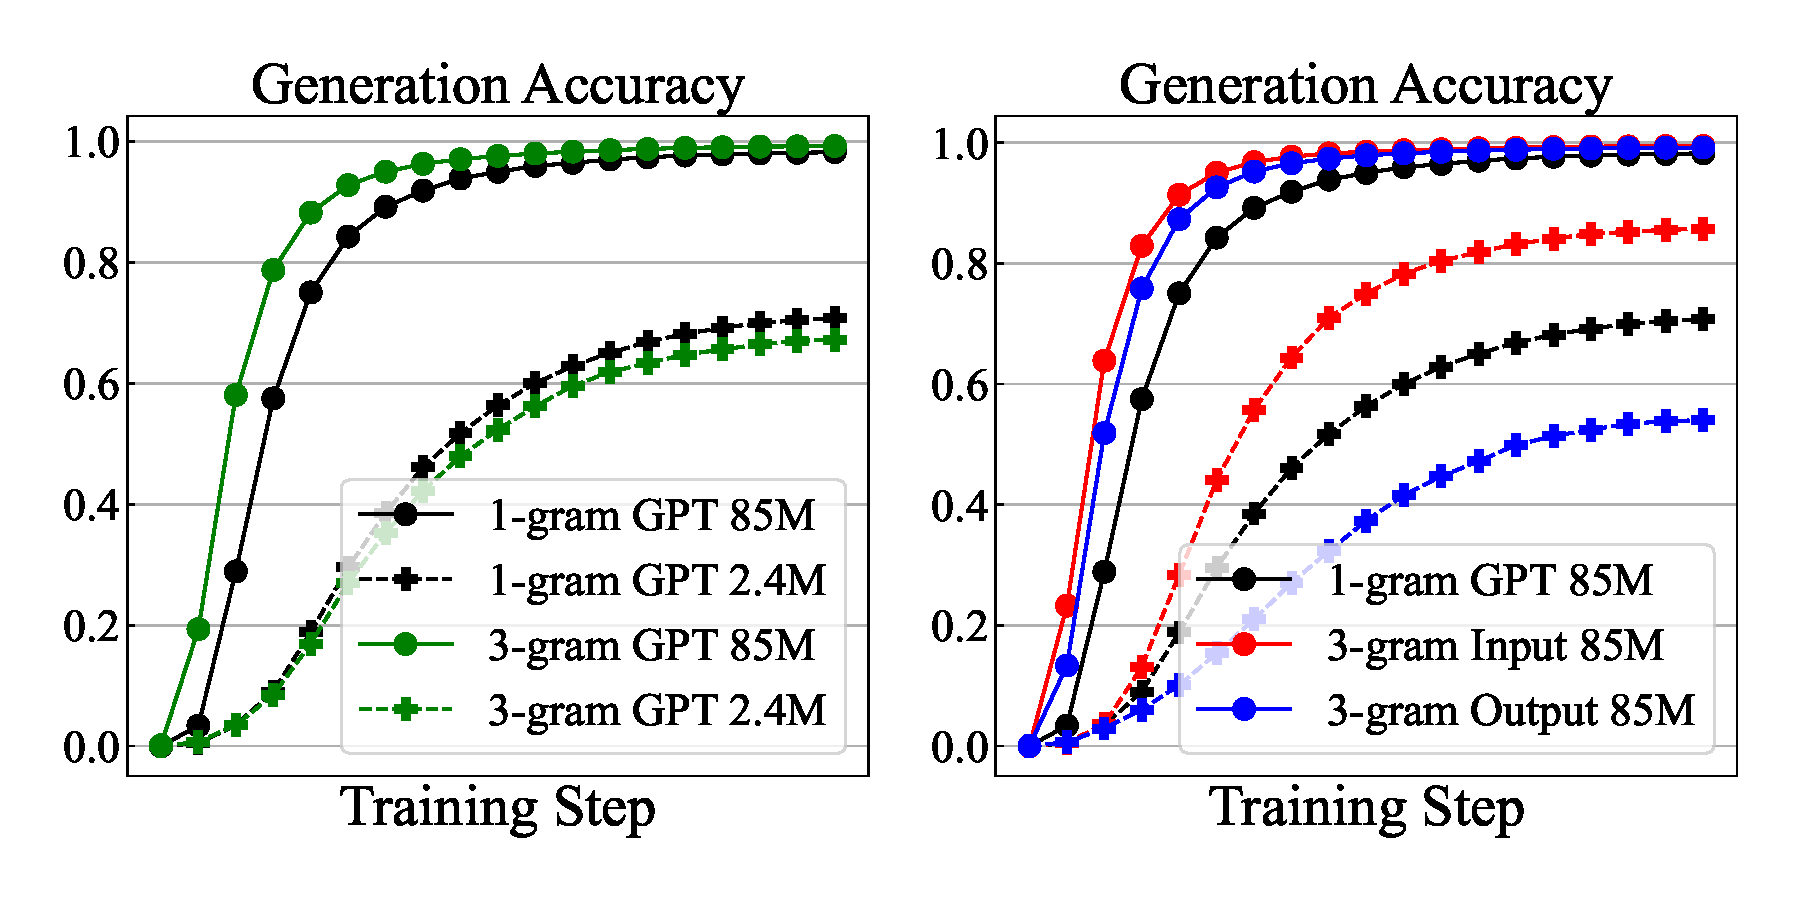
\includegraphics[width=0.96\linewidth]{figures/cfg_tkn_overtkn_exps.pdf}

    \caption{Performance comparison for models trained on CFG data. The left panel compares 1-gram and 3-gram tokenizers, showing that 3-gram improves larger (85M parameters) models but harms smaller (2.4M parameters) ones. The right panel examines 3-gram usage in encoders and decoders, revealing consistent gains with 3-gram encoders regardless of model size, while 3-gram decoders degrade performance in smaller models.}
    \label{fig:cfg_tkn_vs_modelsize_cmp}
\end{figure}

We initiate our research on tokenizers on a synthetic language modeling task to investigate their impact on model performance. 

Following the experimental setup in the previous study~\cite{allenzhu2024physicslanguagemodels1}, we employ a Context-Free Grammar (CFG) as the target language to generate sequences composed of 3 distinct characters, with sequence lengths up to 729. With this setup, the ground-truth language distribution is completely known, enabling precise evaluation of the language models. 
We train GPT-2 models~\cite{radford2019language} of various sizes on CFG-generated samples using next-token prediction loss and evaluate them based on the accuracy of model-generated sequences, which measures the proportion of valid generations. Additional details regarding the experimental setup can be found in Appendix~\ref{sec:appendix_detailed_exp_setup_cfg}.

Our first experiment aims to compare the performance of language models using tokenizers with varying levels of granularity. A baseline tokenizer constructs a vocabulary using the three terminal characters defined by the CFG, tokenizing sentences character-wisely, which we refer as a 1-gram tokenizer. We further define $n$-gram tokenizers, whose vocabulary comprises all $3^n$ possible combinations of $n$ sequential characters. We train both larger and smaller GPT-2 models using 1-gram and 3-gram tokenizers, respectively.

As illustrated in the left panel of~\figref{fig:cfg_tkn_vs_modelsize_cmp}, we observe that a larger tokenizer improves the performance of larger models but negatively impacts smaller models. Notably, larger tokenizers result in shorter training sequences, which significantly reduces training cost. Thus, training larger models with a 3-gram tokenizer not only reduces training costs but also enhances model performance. An intuitive insight is that larger models benefit from larger vocabularies, improving both training efficiency and performance. This finding is also supported by previous studies~\cite{tao2024scaling}.



\begin{figure}
    \centering
    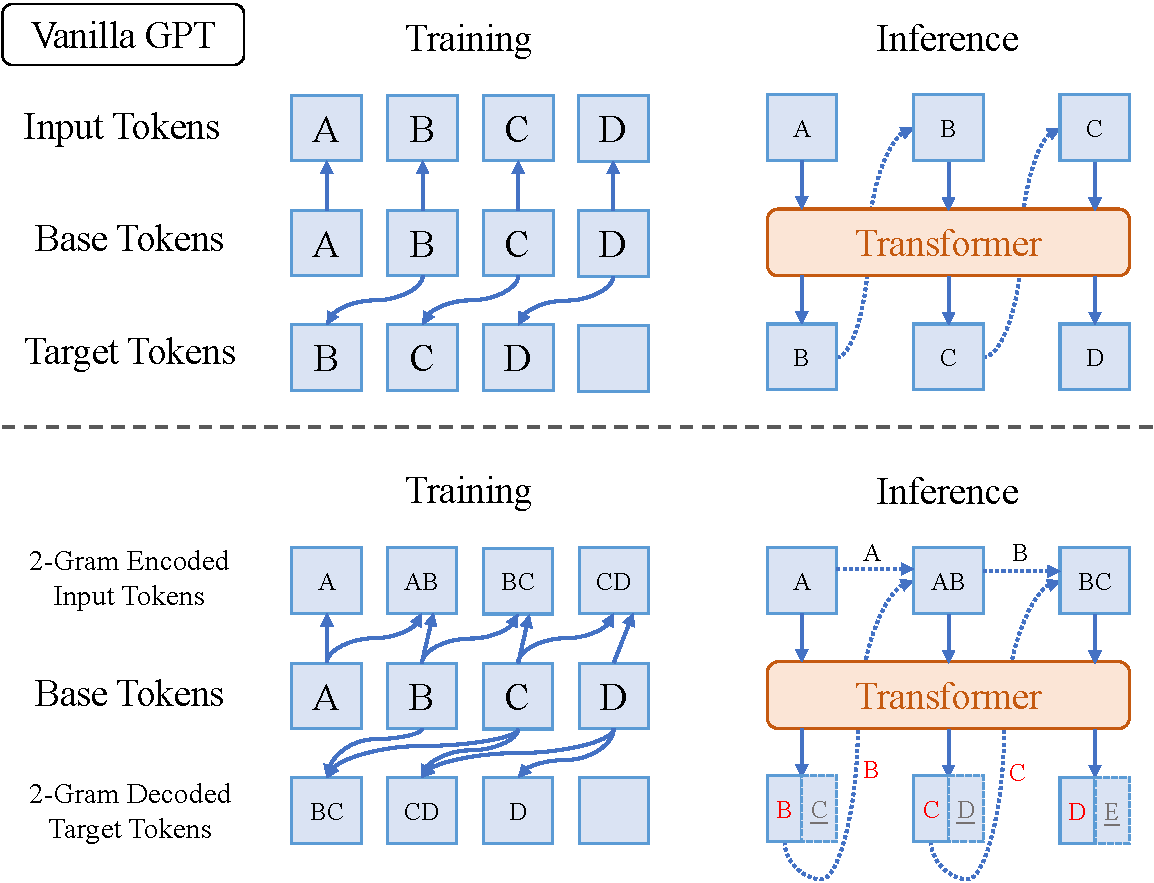
\includegraphics[width=0.96\linewidth]{figures/fig_ideal_over_tkn.pdf}
    \caption{Illustration of 2-gram encoding/decoding GPT. Note that 2-gram decoding only preserves the predicted next 1 token though next 2 is predicted, which keeps inference cost identical to the vanilla model. }
    \label{fig:idea_over_tkn_overview}
\end{figure}


To decouple the influences of enlarging input and output vocabularies, we separately introduce $n$-gram encoding and decoding models, as illustrated in~\figref{fig:idea_over_tkn_overview}. To begin, the raw text is tokenized character-wisely via 1-gram tokenizer. In the $n$-gram encoding model, input tokens are converted to $n$-gram tokens at the input layer, making a large input vocabulary of size $3^n$, and the unembedding layer remains 1-gram, predicting next one character. In the $n$-gram decoding model, the input remains 1-gram tokens while the target labels (i.e., the next token) are converted to $n$-gram labels, resulting a fine-grained classification head that predicts the conditional joint distribution of next $n$ tokens. Note that the training sequence length remains unchanged and matches the length produced by the 1-gram tokenizer for both variants. 

To maintain comparable inference costs, the $n$-gram output model does not generate $n$ tokens simultaneously. Instead, it samples an $n$-gram prediction but preserves the next 1 token only, disregarding extra token predictions during inference. The results for $n=3$ of the two variants are shown in the right panel of \figref{fig:cfg_tkn_vs_modelsize_cmp}. We find that the two models exhibit different behaviors. The 3-gram encoding model consistently enhances performance across all model sizes. However, the 3-gram decoding model improves performance for larger models but degrades it for smaller ones. 

We conclude that, when using large tokenizers, the large input vocabulary is always positive while the large output vocabulary can be negative for smaller models. We hypothesize that the difference lies in their respective roles: the input embedding is responsible for encoding the context into feature embeddings, where a larger vocabulary enhances the representational capacity of the feature mapping, thereby positively impacting the model. In contrast, the output vocabulary determines the granularity of the prediction task. A larger output vocabulary implies more fine-grained supervision signals, which can either be beneficial (e.g., for large models prone to overfitting) or burdensome (e.g., for smaller models suffering from severe underfitting).
Motivated by this observation, we extend our exploration to over-tokenized transformers in real-world natural language modeling.

\subsection{Over-Tokenized Transformer}

Above all, we use a standard natural language tokenizer as the base tokenizer. Then, the challenge arises: if the base tokenizer has a vocabulary size of $V$, which is usually as large as $10^5$, the $n$-gram vocabulary with a size of $V^n$ becomes exceedingly large and impractical. To address this, we propose approximating the large embedding table through a series of matrix decompositions.

Given a sequence of input ids $x_1,x_2,\dots,x_t$ from the base tokenizer, we define the $n$-gram input token $x^{(-n)}_i$  as follows:
\begin{align}
    x^{(-n)}_i = f(x_i,x_{i-1},\dots,x_{i-n+1}),
\end{align}
where $f(z_1, ..., z_n)$ is an index mapping function, and out-of-range indices are padded with zero tokens, \ie, $x_i = 0, \forall i \not\in [1, t]$. One intuitive design treats $(z_1, \dots, z_n)$ as a $p$-base number, defining  $f$ as 
\begin{equation}
    f(z_1, ..., z_n) = \sum_{i=1}^{n} z_i p^{i-1}, \label{eq:index_mapping_func}
\end{equation} 
where $p \geq V$ ensures that $f$ is a bijection. Typically, $p$ is set to $V$ to keep the range of $f$ as compact as possible. Notably, $x^{(-1)}_i = x_i$ corresponds to the standard transformer input.

\paragraph{General $n$-gram Embedder.} The key to designing an flexible $n$-gram embedder module is to make the vocabulary size configurable. We achieve this efficiently using a simple tiled matrix parameterization approach. Specifically, the tiled matrix parameterization extends an $m \times d$ embedding table into a $V^n \times d$ embedding table by tiling, where $m$ is a configurable size. In practice, the lookup process is straightforward: an input token $x^{(n)}$ is mapped by taking its modulus with respect to $m$. In summary, our $n$-gram embedder is formalized as
\begin{align}
    \mathbf{h}=\mathbf{E}\left(x^{(n)}\ \%\ m\right),
\end{align}
where $\mathbf{h}$ is the output embedding, $\mathbf{E} \in \mathbb{R}^{m \times d}$ is the embedding matrix, and $\%$ is the modulo operation. We denote this $n$-gram $m \times d$ embedder as $\mathbb{E}^{m \times d}(x^{(n)})$. This $n$-gram hashing technique is commonly used in previous works~\cite{huang21f_interspeech, roy2022ngrammeraugmentingtransformerslatent}.



\paragraph{Over-Encoding(OE).} We find a hierarchical encoding paradigm to be highly effective. Specifically, we compute the input embedding to the GPT model as the sum of 1-, 2-, ..., $n$-gram embeddings. Additionally, we observe further benefits from using smaller embedding dimensions. An embedder $\mathbb{E}^{m \times d}_n$ can be sliced into $k$ low-rank decomposed embedders, represented as:
\begin{equation}
    \mathbb{E}^{m\times d|k}(x^{(-n)}) = \sum_{i=1}^k\mathbb{E}^{m\times \frac{d}{k}}_i(x^{(-n)})\mathbf{W}_i,
\end{equation}
where $\mathbf{W}_i \in \mathbb{R}^{\frac{d}{k} \times d_{model}}$ projects the embedding vector to match the model dimension. Using the same number of embedding parameters and incurring only minimal additional cost through $k$ dense matrices $\mathbf{W}_i \in \mathbb{R}^{\frac{d}{k} \times d_{model}}$, this approach significantly enhances performance. 

Overall, the over-encoding process maps an input token to an embedding as follows:
\begin{align}
    \texttt{OE}(x)= \mathbb{E}^{V\times d}(x^{(-1)}) +\sum_{i=2}^{n} \mathbb{E}^{m\times \frac{d}{n}|k}(x^{(-i)}), \label{eq:oe_standard}
\end{align}
where the 1-gram embedding $\mathbb{E}^{V \times d}(x^{(-1)})$ is implemented consistently with the original Transformer to align with the tied weight design. Generally, $m$ is set to a value much larger than $V$, and the model performance is observed to improve consistently as $m$ increases. 

Notably, for multiple embedders with $m$ rows, minor adjustments (\eg, replacing $m$ with $m+2$) are made to ensure each embedder has a unique mapping. This increases the combinatorial capacity of the embedding; otherwise, the slice trick would make no difference.
A detailed pytorch-like implementation for OE can be found in Appendix~\ref{sec:implementation}.

We also acknowledge a concurrent work, BLT~\cite{pagnoni2024bytelatenttransformerpatches}, which employs a similar $n$-gram hashing embedding strategy for byte-level tokens.

\paragraph{Over-Decoding(OD).} Based on the conclusions from our CFG experiments, decoding additional tokens is only effective for sufficiently large models. As a matter of fact, previous researches on Multi-Token Prediction (MTP)~\cite{gloeckle2024better} are typically approximations of over-decoding, and share the same conclusion that only large models benefit from future token predictions. Generally, MTP-like methods are viewed as over-decoding in this paper. In addition, we explore other solutions for over-decoding in Appendix~\ref{appendix:od} for reference.

\paragraph{Over-Tokenized Transformer(OT).} Integrating over-encoding and over-decoding, we obtain over-tokenized transformer. Specifically, we focus on the conditional recursive form of MTP proposed in DeepSeek V3~\cite{deepseekai2024deepseekv3technicalreport}, which we refer as MTP-DS. In this formulation, MTP no longer predicts the next few tokens in parallel but instead predicts them sequentially. For the $n$-th head, the embedding of the next $(n-1)$-th token is concatenated to the layer input as a condition for the next $n$-th token prediction. 

Under MTP-DS architecture, over-encoding enhances the representation capacity of token embeddings and directly participates future token predictions. On the one hand, the future token prediction tasks become easier to learn. On the other hand, the over-encoding can be trained more sufficiently. With these advantages, the integration of the two methods yields greater benefits, even on relatively smaller models.


\subsection{Engineering Challenges and Solutions} 

The over-encoding constructs a very large input vocabulary. In theory, as the embeddings are sparsely accessed based on token ids, enlarging vocabulary should barely impact the training or inference cost. However, the large embedding parameters can place substantial memory pressure on GPUs. Furthermore, when parameter sharding strategies, such as FSDP~\cite{zhao2023pytorch}, are applied during training, the communication of these sparse parameters can severely degrade training efficiency, further constraining the choice of $m$ (the vocabulary size) to smaller values.

To mitigate this issue, we recommend using tensor parallelism specifically for the over-encoding embedding layer to reduce communication overhead. The embedding table is row-wise sharded across all data-parallel (DP) ranks. For a given input, the token is sent to the corresponding DP rank that holds its embedding, queried for the embedding vector, and then the resulting embedding is sent back to the original DP rank. This process involves two all-to-all communications during the forward pass and one all-to-all communication during the backward pass, resulting in a total communication volume significantly lower than that of FSDP.

We implement this optimization and find that training an over-encoded model with $m = 10^7$ on FSDP reduces throughput by less than 5\%. In contrast, without this optimization, FSDP experiences a 25\% slowdown and easily runs out of memory for vocabulary sizes exceeding $m = 5 \times 10^6$.

We believe that the current implementation still does not represent the limit of over-encoding performance optimization. Its greatest advantage is that the vocabulary input is decoupled from the model architecture. This decoupling allows the embedding lookup for the next micro-batch to be performed in advance. For example, we can design a dedicated embedding lookup stage in a pipeline-parallel training framework, which overlaps the communication required for embedding lookups with the transformer forward of the current micro-batch. This strategy would maintain training throughput without any performance degradation. 
Additionally, under this approach, the over-encoding parameters could be offloaded to the CPU, completely alleviating GPU memory pressure. Notably, similar training frameworks have already been implemented~\cite{fang2022frequency, colossal-ai}. Over-Encoding could leverage these designs to improve model performance with minimal additional cost.
